\documentclass{article}

% if you need to pass options to natbib, use, e.g.:
%     \PassOptionsToPackage{numbers, compress}{natbib}
% before loading neurips_2025

% The authors should use one of these tracks.
% Before accepting by the NeurIPS conference, select one of the options below.
% 0. "default" for submission
% \usepackage{neurips_2025}
% the "default" option is equal to the "main" option, which is used for the Main Track with double-blind reviewing.
% 1. "main" option is used for the Main Track
%  \usepackage[main]{neurips_2025}
% 2. "position" option is used for the Position Paper Track
%  \usepackage[position]{neurips_2025}
% 3. "dandb" option is used for the Datasets & Benchmarks Track
 % \usepackage[dandb]{neurips_2025}
% 4. "creativeai" option is used for the Creative AI Track
%  \usepackage[creativeai]{neurips_2025}
% 5. "sglblindworkshop" option is used for the Workshop with single-blind reviewing
 % \usepackage[sglblindworkshop]{neurips_2025}
% 6. "dblblindworkshop" option is used for the Workshop with double-blind reviewing
%  \usepackage[dblblindworkshop]{neurips_2025}

% After being accepted, the authors should add "final" behind the track to compile a camera-ready version.
% 1. Main Track
% \usepackage[main, final]{neurips_2025}
% 2. Position Paper Track
%  \usepackage[position, final]{neurips_2025}
% 3. Datasets & Benchmarks Track
 % \usepackage[dandb, final]{neurips_2025}
% 4. Creative AI Track
%  \usepackage[creativeai, final]{neurips_2025}
% 5. Workshop with single-blind reviewing
%  \usepackage[sglblindworkshop, final]{neurips_2025}
% 6. Workshop with double-blind reviewing
%  \usepackage[dblblindworkshop, final]{neurips_2025}
% Note. For the workshop paper template, both \title{} and \workshoptitle{} are required, with the former indicating the paper title shown in the title and the latter indicating the workshop title displayed in the footnote.
% For workshops (5., 6.), the authors should add the name of the workshop, "\workshoptitle" command is used to set the workshop title.
% \workshoptitle{WORKSHOP TITLE}

% "preprint" option is used for arXiv or other preprint submissions
\usepackage[preprint]{neurips_2025}

% to avoid loading the natbib package, add option nonatbib:
% \usepackage[nonatbib]{neurips_2025}

\usepackage[utf8]{inputenc} % allow utf-8 input
\usepackage[T1]{fontenc}    % use 8-bit T1 fonts
\usepackage{hyperref}       % hyperlinks
\usepackage{url}            % simple URL typesetting
\usepackage{booktabs}       % professional-quality tables
\usepackage{amsfonts}       % blackboard math symbols
\usepackage{nicefrac}       % compact symbols for 1/2, etc.
\usepackage{microtype}      % microtypography
\usepackage{xcolor}         % colors
\usepackage{graphicx}
\usepackage{float}
\usepackage{amsmath}
\usepackage{tikz}
\usetikzlibrary{arrows.meta,positioning,fit,calc,decorations.pathreplacing}

% Note. For the workshop paper template, both \title{} and \workshoptitle{} are required, with the former indicating the paper title shown in the title and the latter indicating the workshop title displayed in the footnote. 
\title{Proposal: Factorized Innovation Spike-Coding for Local, Adaptive Estimation}

% The \author macro works with any number of authors. There are two commands
% used to separate the names and addresses of multiple authors: \And and \AND.
%
% Using \And between authors leaves it to LaTeX to determine where to break the
% lines. Using \AND forces a line break at that point. So, if LaTeX puts 3 of 4
% authors names on the first line, and the last on the second line, try using
% \AND instead of \And before the third author name.

\author{%
  Berke Altiparmak \\
  MS in Data Science\\
  Harvard University\\
  %
}


\begin{document}


\maketitle

\begin{abstract}
We propose a spiking, fully-local estimator that merges the closed-form spiking control architecture of spike coding networks (SCNs) with the strictly local, innovation-driven learning rules of neural optimal feedback control (Bio-OFC). The key technical device is a factorization of the Kalman correction into two learnable pathways: spikes$\to$predicted-sensor and innovation$\to$state. This makes all plasticity synapse-local while retaining SCN's sparse, efficient spiking substrate. This note summarizes the prior architectures and motivates why naive "add local learning to SCN" fails, then presents our architecture in detail.
\end{abstract}

This is a summary prepared for Prof. Cengiz Pehlevan on 20 Nov 2026.

\section{Background: Spike Coding Networks (SCN)}
\paragraph{Architecture.}
SCNs implement linear dynamics and LQG-like correction in a recurrent spiking network whose decoded activity estimates the latent state. Let $s(t)\in\mathbb{R}^N$ be spikes and $r$ the filtered traces, $\dot r=-\lambda r + s$. A fixed decoder $D\in\mathbb{R}^{K\times N}$ yields $\hat x = D r$. 

Two recurrent pathways shape dynamics:
\begin{align}
\underbrace{\Omega_f}_{\text{fast}} = -D^\top D \quad\text{(lateral reset/competition)}, \qquad
\underbrace{\Omega_s}_{\text{slow}} = D^\top (A+\lambda I) D \quad\text{(internal model)}.
\end{align}


Membrane voltages evolve as
\begin{align}
\dot v = -\lambda v + \Omega_s r + \Omega_f s + \underbrace{F_k y + \Omega_k r}_{\text{Kalman-style correction}},
\end{align}
so that voltages encode a population prediction error and spikes are greedy error-reducing events. In the closed-form SCN-LQG construction, the correction blocks are
\begin{align}
F_k = D^\top K_f, \qquad \Omega_k = -D^\top K_f C D,
\end{align}
which assume known plant/observation matrices $(A,B,C)$ and Kalman gain $K_f$.

\paragraph{Strengths/limits.}
SCNs give an analytic, sparse spiking realization of linear estimation/control, with robustness to dropout and noise and no training once $(A,B,C,K_f)$ are identified. However, the Kalman blocks are fixed: there is no online, biologically local learning of $C$ or $K_f$ inside the spiking substrate.

\section{Background: Neural Optimal Feedback Control with Local Learning (Bio-OFC)}
\paragraph{Architecture.}
Bio-OFC casts estimation as predict $\to$ compare $\to$ correct using an innovation $e = y - C\hat x$ and shows that one can learn the observation map and Kalman-like gain with strictly local rules:
\begin{align}
\Delta \hat C \propto e\,\hat x^\top,\quad
\Delta \hat L \propto (L e)\, e^\top,\quad
\Delta \hat A \propto (L e)\,\hat x^\top,
\end{align}
where $Le$ is the postsynaptic innovation current. Sensory delay is handled by delay-matching the prediction pathway, so the same circuit computes $e_t = y_{t+1-\tau}-\hat y_{t+1-\tau}$ without replay.

\paragraph{Strengths/limits.}
These rules are local (pre-trace $\times$ postsyn current, plus optional global scalar) and learn $C$, $L$ (Kalman gain), and $A$ online. But the original instantiation is not built on the SCN spiking substrate (no $\Omega_f$ fast resets, no sparse spike coordination), and thus it does not automatically inherit SCN's coding efficiency and robustness.

\section{Why naive ``SCN + local learning'' does not work}
A tempting approach is: keep the SCN equations and just replace the fixed correction blocks with learned weights via Hebbian/three-factor rules. During one of our meetings, we talked about a critical issue: nonlocal matrix structures.

The SCN correction contains the composite ${-D^\top K_f C D}$. Learning this composite directly would require access to transposes/inverses or backpropagated errors that are not locally available at any single synapse.

Without architectural changes, the SCN estimator does not expose the right local teaching signals to each synapse.

\section{Proposal: Factorized Innovation Spike-Coding (FISC)}
\subsection{Core idea: factorize the Kalman correction (what changes and why it matters)}
\label{sec:factorization}

\paragraph{SCN's original Kalman-style correction.}
In the SCN construction, the (continuous-time) estimator voltage receives two correction terms:
\[
\dot v \;=\; -\lambda v \;+\; \underbrace{\Omega_s r + \Omega_f s}_{\text{predict}} \;+\; \underbrace{F_k\,y \;+\; \Omega_k\, r}_{\text{correct}},
\]
with fixed matrices (once the plant is identified)
\[
\boxed{F_k^{\text{(SCN)}} = D^\top K_f}, 
\qquad
\boxed{\Omega_k^{\text{(SCN)}} = -\,D^\top K_f C D}.
\]
Here $r\in\mathbb{R}^N$ are filtered spikes, $y\in\mathbb{R}^Q$ are sensors, $D\in\mathbb{R}^{K\times N}$ is the decoder, $C\in\mathbb{R}^{Q\times K}$ is the observation matrix, and $K_f\in\mathbb{R}^{K\times Q}$ is the Kalman gain. This realizes the Kalman innovation step in spikes, but assumes $C$ and $K_f$ are known and not learned online.

\paragraph{Our factorization.}
We replace the composite SCN block $(-D^\top K_f C D)$ by two learnable maps and a computed residual:
\[
\underbrace{\hat y = W_y\, r}_{\text{learned: spikes}\to\text{predicted sensor}}, 
\qquad
\underbrace{e = y - \hat y}_{\text{computed residual (innovation)}}, 
\qquad
\underbrace{G e}_{\text{learned: innovation}\to\text{state correction}}.
\]
This yields learned correction blocks
\[
\boxed{F_k \;\equiv\; G}, 
\qquad
\boxed{\Omega_k \;\equiv\; -\,G\,W_y}.
\]
Plugging back into the voltage dynamics gives
\[
\dot v \;=\; -\lambda v \;+\; \Omega_s r + \Omega_f s \;+\; G y \;+\; (-GW_y)\, r.
\]
At convergence, if $W_y \!\to\! C D$ and $G \!\to\! D^\top K_f$, we recover SCN exactly:
\[
G y + (-GW_y) r \;\to\; D^\top K_f\, y \;-\; D^\top K_f C D\, r \;\equiv\; F_k^{\text{(SCN)}} y + \Omega_k^{\text{(SCN)}} r.
\]

\paragraph{Why factorization is the key to strict locality.}
The composite $-D^\top K_f C D$ entangles state$\to$sensor ($C D$) and sensor$\to$state ($D^\top K_f$). Learning it directly would require nonlocal information (e.g., $C^\top$ or transposes of $D$). Factorization exposes two synapse-specific maps that can each be updated with local signals:
  \[
  \Delta W_y \;\propto\; e\, r^\top \quad(\text{pre: $r$, post-error: $e$}), 
  \qquad
  \Delta G \;\propto\; (G e)\, e^\top \quad(\text{pre: $e$, post: innovation current $Ge$}).
  \]
  The slow predictor updates locally as well:
  \[
  \Delta \Omega_s \;\propto\; (G e)\, r^\top \quad(\text{pre: $r$, post: $Ge$ on the prediction dendrite}).
  \]

\subsection{Populations and wiring (architecture)}
\label{sec:arch}

We instantiate three interacting populations with clear roles and strictly local learning at their synapses. Throughout, $K$ is the latent state dimension, $Q$ the number of sensor channels, and $N$ the size of the spiking estimator code (often $N\ge K$ for overcomplete sparse coding).

\paragraph{Signals and shapes (at a glance).}
\begin{itemize}
\item Estimator spikes/traces: $s(t)\in\mathbb{R}^N$, $r(t)\in\mathbb{R}^N$, with $\dot r=-\lambda r+s$.
\item State estimate (decoded): $\hat x(t)=D\,r(t)$, with $D\in\mathbb{R}^{K\times N}$ (fixed decoder).
\item Predicted sensors: $\hat y(t)=W_y\,r(t-\tau)$, with $W_y\in\mathbb{R}^{Q\times N}$ (learned).
\item Innovation (residual): $e(t)=y(t)-\hat y(t)\in\mathbb{R}^Q$.
\item Innovation current into estimator: $Ge(t)$ with $G\in\mathbb{R}^{N\times Q}$ (learned).
\item Recurrent matrices inside estimator: $\Omega_f=-D^\top D\in\mathbb{R}^{N\times N}$ (fast competition/reset), $\Omega_s\in\mathbb{R}^{N\times N}$ (slow internal model; learned).
\end{itemize}

\paragraph{(A) Estimator population \textbf{E} (spiking; $N$ neurons).}
\emph{Role:} represent $\hat x$ and implement predict+correct. Each neuron has two dendritic compartments:
\begin{align}
\dot v &= -\lambda v 
\;+\; \underbrace{\Omega_s r + \Omega_f s}_{\text{prediction dendrite}}
\;+\; \underbrace{G e}_{\text{innovation dendrite}}
\;+\; \eta, 
\qquad
\hat x = D r,\quad \dot r=-\lambda r+s.
\end{align}
The fast path $\Omega_f=-D^\top D$ yields coordinated, sparse, greedy error-reducing spikes; the slow path $\Omega_s$ carries the internal linear predictor (learned online). The innovation dendrite receives $Ge$, a low-dimensional corrective current.

\paragraph{(B) Prediction population \textbf{P} (linear or spiking; $Q$ units).}
\emph{Role:} predict what sensors should report from the current code:
\begin{align}
\hat y(t)=W_y\,r(t-\tau), \qquad W_y\in\mathbb{R}^{Q\times N}.
\end{align}
The delay line (or eligibility trace) on $r$ aligns prediction with sensor latency $\tau$. Learning at $E\!\to\!P$ synapses is strictly local, using the per-channel innovation $e_k$ as a postsynaptic error:
\begin{align}
\Delta W_y \propto e\,r^\top \quad \text{(pre: $r_j$, post-error: $e_k$).}
\end{align}

\paragraph{(C) Innovation population \textbf{\(\varepsilon\)} (linear or spiking; $Q$ units).}
\emph{Role:} compute the innovation and broadcast it:
\begin{align}
e(t)=y(t)-\hat y(t), \qquad \hat y=W_y r(t-\tau).
\end{align}
$\varepsilon$ receives excitatory input from sensors $y$ and opposing input from $P$. It projects $e$ to the estimator via $G$, and also serves as the local teacher for $W_y$.
Learning at $\varepsilon\!\to\!E$ synapses is local, using presynaptic $e_k$ and postsynaptic innovation current $(Ge)_i$:
\begin{align}
\Delta G \propto (G e)\, e^\top \quad \text{(pre: $e_k$, post: $(Ge)_i$).}
\end{align}

\paragraph{Local learning for the internal predictor in \textbf{E}.}
The slow recurrent synapses in \textbf{E} update by pairing presynaptic $r_j$ with the postsynaptic innovation current $(Ge)_i$ on the prediction dendrite:
\begin{align}
\Delta \Omega_s \propto (G e)\, r^\top.
\end{align}
All three learning rules are three-factor and synapse-local: (presynaptic eligibility trace) $\times$ (postsynaptic dendritic current) $\times$ (optional scalar neuromodulatory gate).

\paragraph{Factorized correction embeds SCN Kalman blocks.}
With $\hat y=W_y r$ and $Ge$ injected on the innovation dendrite, the correction decomposes as
\[
F_k \equiv G,\qquad \Omega_k \equiv -GW_y,
\]
so the estimator voltage receives $Gy - GW_y r$. At convergence ($W_y\!\to\!CD$, $G\!\to\!D^\top K_f$), this reproduces $D^\top K_f\,y - D^\top K_f C D\, r$ from SCN.

\paragraph{Delay alignment (local).}
A synaptic delay (or matched eligibility trace) on the $r\!\to\!\hat y$ path ensures $e(t)=y(t)-W_y r(t-\tau)$ is computed channel-wise and locally. The same $e(t)$ gates all plasticity; no global buffers or replay are needed.

\paragraph{Why this architecture is local.}
Each plastic synapse uses only: (i) its own presynaptic trace ($r_j$ or $e_k$), (ii) its own postsynaptic dendritic current ($(Ge)_i$ on \textbf{E} or $e_k$ on \textbf{P}/\(\varepsilon\)), plus (iii) an optional broadcast scalar. No transposes, inverses, or messages from other postsynaptic neurons are required.

\begin{figure}[t]
\centering
\resizebox{\linewidth}{!}{%
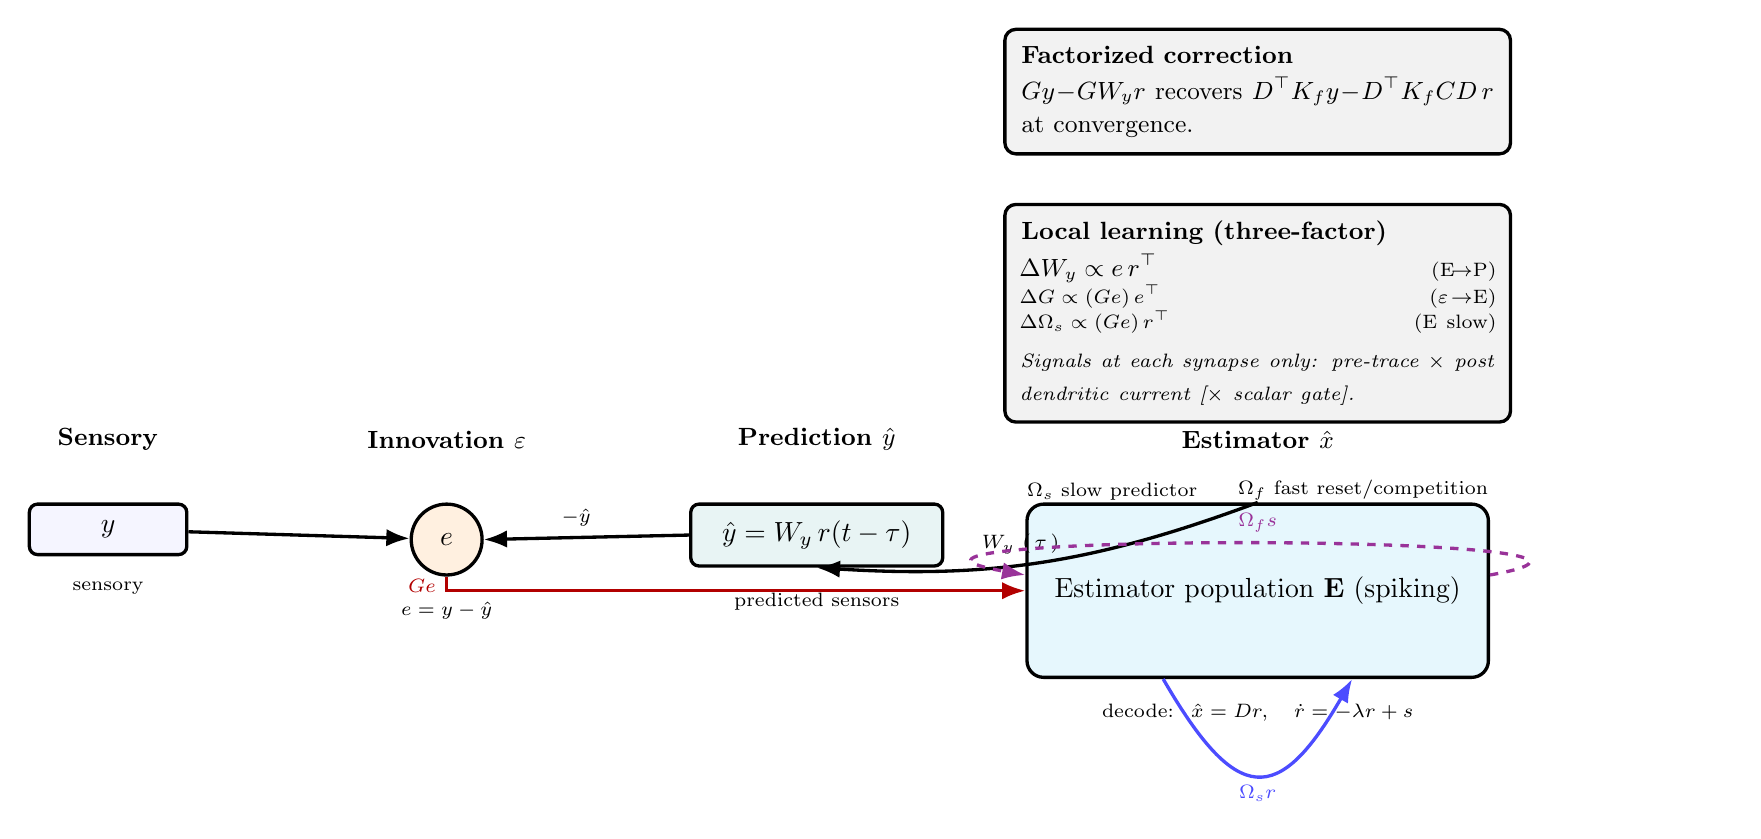
\begin{tikzpicture}[>=Latex, node distance=16mm and 18mm,
  every node/.style={transform shape}] % keep proportions under resize

  % ===== Styles =====
  \tikzset{
    arrow/.style={-Latex, very thick},
    box/.style={draw, rounded corners=3pt, very thick, inner sep=6pt, align=center, fill=blue!4},
    bubble/.style={circle, draw, very thick, inner sep=3pt, minimum size=9mm, align=center, fill=orange!12},
    pop/.style={draw, rounded corners=6pt, very thick, inner sep=10pt, align=center, fill=cyan!10, minimum width=50mm, minimum height=22mm},
    panel/.style={draw, rounded corners=4pt, very thick, inner sep=6pt, align=left, fill=gray!10},
    smallcap/.style={font=\scriptsize, align=center},
    tinycap/.style={font=\scriptsize, align=left}
  }

  % ===== Column anchors (fixed grid so nothing drifts) =====
  % Horizontal spacing is fixed; everything is placed relative to these.
  \coordinate (C1) at (0,0);        % Sensory
  \coordinate (C2) at (4.3,0);      % Innovation
  \coordinate (C3) at (9.0,0);      % Prediction
  \coordinate (C4) at (14.6,0);     % Estimator

  % Headings on one baseline
  \node[font=\small] at (C1) {\textbf{Sensory}};
  \node[font=\small] at (C2) {\textbf{Innovation $\varepsilon$}};
  \node[font=\small] at (C3) {\textbf{Prediction $\hat y$}};
  \node[font=\small] at (C4) {\textbf{Estimator $\hat x$}};

  % ===== Row of main nodes (aligned under headings) =====
  \node[box, minimum width=20mm, below=8mm of C1] (Y) {$y$};
  \node[bubble, below=8mm of C2] (Eps) {$e$};
  \node[box, fill=teal!9, minimum width=32mm, below=8mm of C3] (Pred) {$\hat y = W_y\, r(t-\tau)$};
  \node[pop, below=8mm of C4] (Est) {Estimator population \textbf{E} (spiking)}; % estimator box (blue)

  % Captions (separate nodes; no overlaps)
  \node[smallcap, below=2mm of Y] {sensory};
  \node[smallcap, below=2mm of Eps] {$e = y - \hat y$};
  \node[smallcap, below=2mm of Pred] {predicted sensors};
  \node[tinycap, below=2mm of Est] {decode: $\ \hat x = D r,\quad \dot r = -\lambda r + s$};

  % Internal annotations (kept outside the box interior)
  \node[tinycap, above right=-1mm and -1mm of Est.north west] {$\Omega_s$ slow predictor};
  \node[tinycap, above left=-1mm and -1mm of Est.north east] {$\Omega_f$ fast reset/competition};

  % ===== Connections =====
  \draw[arrow] (Y) -- (Eps);
  \draw[arrow] (Pred.west) -- node[above, pos=.55, font=\scriptsize] {$-\hat y$} (Eps.east);
  \draw[arrow, red!70!black] (Eps.south) |- node[left, pos=.33, font=\scriptsize] {$G e$} (Est.west);
  \draw[arrow] (Est.north) to[bend left=12] node[above, pos=.55, font=\scriptsize] {$W_y$ (\,$\tau$\,)} (Pred.south);

  % Schematic loops (kept low and high to avoid captions)
  \draw[->, very thick, blue!70] ([xshift=-12mm]Est.south) to[out=-60,in=-120, looseness=2] node[below, font=\scriptsize] {$\Omega_s r$} ([xshift=12mm]Est.south);
  \draw[->, very thick, violet!80, dashed] ([yshift=2mm]Est.east) to[out=10,in=170, looseness=1.35] node[above, font=\scriptsize] {$\Omega_f s$} ([yshift=2mm]Est.west);

  % ===== Panels stacked ABOVE estimator (fits page width) =====
  \node[panel, text width=60mm, above=10mm of Est.north] (Rules) {\small
    \textbf{Local learning (three-factor)}\\[2pt]
    $\Delta W_y \propto e\, r^{\top}$ \hfill \scriptsize(E$\!\to$P)\\
    $\Delta G \propto (G e)\, e^{\top}$ \hfill \scriptsize($\varepsilon\!\to$E)\\
    $\Delta \Omega_s \propto (G e)\, r^{\top}$ \hfill \scriptsize(E slow)\\[2pt]
    \emph{Signals at each synapse only: pre-trace $\times$ post dendritic current [$\times$ scalar gate].}
  };

  \node[panel, text width=60mm, above=6mm of Rules] (Fact) {\small
    \textbf{Factorized correction}\\[1pt]
    $G y - G W_y r$ recovers $D^{\top} K_f y - D^{\top} K_f C D\, r$ at convergence.
  };

\end{tikzpicture}%
} % end resizebox
\caption{\textbf{FISC architecture}. Sensory measurements \(y\) are compared with predicted sensors \(\hat y = W_y\,r(t-\tau)\) to form the innovation \(e = y-\hat y\).
The innovation drives a low-dimensional corrective current \(G e\) into the estimator population \textbf{E}, which encodes the state via sparse spikes with a slow internal model \(\Omega_s r\) and a fast reset/competition path \(\Omega_f s\); the decoded estimate is \(\hat x = D r\).
This factorized correction \(G y - G W_y r\) recovers the SCN Kalman blocks \(D^\top K_f y - D^\top K_f C D\,r\) at convergence.
All learning is strictly local and three-factor.}

\end{figure}


\subsection{Local learning rules (three-factor, synapse-local)}
\label{sec:derivation}

We learn by minimizing the innovation energy
\(
\mathcal{L}(t)=\tfrac12\|e(t)\|^2
\)
with
\(
e(t)=y(t)-\hat y(t),\quad \hat y(t)=W_y\,r(t-\tau),\quad \hat x(t)=D r(t).
\)
The estimator dynamics are
\(
\dot v=-\lambda v+\Omega_s r+\Omega_f s+G e,
\)
so the only sensor-dependent current is \(\,Ge\,\) (the innovation current), while \(\Omega_s r\) is the internal predictor.

\paragraph{Assumptions, as standard in local derivations.} .

(i) \emph{Time-scale separation}: synaptic changes are slow vs.\ membrane dynamics, so we use instantaneous (semi-gradient) updates

(ii) \emph{Surrogate gradient} for spikes: treat postsynaptic dendritic currents as the local sensitivity signal

(iii) \emph{Delay matching}: \(\hat y=W_y r(t-\tau)\) so \(e(t)\) uses aligned signals (no replay).

\paragraph{Learning \(W_y\): spikes\(\to\)sensors.}
With \(e=y-W_y r_\tau\) (shorthand \(r_\tau=r(t-\tau)\)),
\[
\frac{\partial \mathcal{L}}{\partial W_y} \;=\; \frac{\partial \tfrac12\|e\|^2}{\partial e}\,\frac{\partial e}{\partial W_y}
\;=\; e\,(-r_\tau)^\top
\;\Rightarrow\;
\Delta W_y \;\propto\; e\,r_\tau^\top.
\]
This is pure pre\(\times\)post (presyn \(r_\tau\), postsyn error \(e\)), with an optional local stabilizer (e.g., Oja/decay).

\paragraph{Learning \(G\): innovation\(\to\)state (Bio-OFC preconditioning, locally).}
Changing \(G\) perturbs the innovation current \(Ge\), which adjusts \(\hat x\) (via spikes) and thereby \(\hat y\) and \(e\).
Direct gradients would require nonlocal transports. Bio-OFC shows one can use the postsynaptic innovation current as a local descent direction:
\[
\Delta G \;\propto\; (Ge)\,e^\top.
\]
This is the spiking-coordinate analogue of Bio-OFC’s \(\Delta L \propto (Le)e^\top\), with the identification \(G \equiv D^\top L\).

Intuitively, if component \(e_k\) is persistently positive and neuron \(i\) receives a corrective current \((Ge)_i\) that reduces the residual, strengthen the synapse \(G_{ik}\).


\paragraph{Learning \(\Omega_s\): internal predictor (SCN map of \(\Delta A\)).}
Bio-OFC’s local system-ID rule updates the latent dynamics as
\(
\Delta A \propto (Le)\,\hat x^\top.
\)
In SCN coordinates \(\Omega_s = D^\top (A+\lambda I) D\), so
\[
\Delta \Omega_s
= D^\top (\Delta A) D
\;\propto\;
(D^\top L e)\,(D^\top \hat x)^\top
\;=\;
(Ge)\,r^\top,
\]
because \(\hat x=Dr\) and \(G\equiv D^\top L\).
Thus the slow E \(\!\leftrightarrow\!\) E synapse learns via presyn \(r\) and the postsynaptic innovation current \((Ge)\), again a strictly local three-factor rule.

\paragraph{Putting it together.}
All three rules share the same structure:
\[
\boxed{\;
\Delta W_y \propto e\,r^\top,\qquad
\Delta G \propto (Ge)\,e^\top,\qquad
\Delta \Omega_s \propto (Ge)\,r^\top
\;}
\]
Each update is computed at the synapse from (i) a presynaptic eligibility trace (either \(r\) or \(e\)), (ii) a postsynaptic dendritic current (the neuron’s own \(Ge\) on \textbf{E}, or \(e\) on \textbf{P}/\(\varepsilon\)), and (iii) an optional scalar neuromodulatory gate (our derivations actually haven't used this one). No transposes, inverses, or messages from other postsynaptic neurons are required.

\paragraph{Why this recovers the SCN Kalman blocks.}
With \(\hat y=W_y r\) and the innovation current \(Ge\) injected on a separate dendrite, the correction is
\(
Gy - GW_y r \equiv F_k y + \Omega_k r
\)
with \(F_k=G\), \(\Omega_k=-GW_y\).
At convergence \(W_y\!\to\!CD\), \(G\!\to\!D^\top K_f\), yielding the original SCN correction \(D^\top K_f y - D^\top K_f C D\, r\) while having learned everything with strictly local plasticity.



\subsection{Summary}
SCN provides the \emph{spiking physics} (sparse, robust coding; $\Omega_f$ competition; $\Omega_s$ prediction). Bio-OFC provides the \emph{innovation calculus} (error nodes and strictly local updates). Our factorization exposes exactly the right local teaching signals to each synapse: $W_y$ learns \emph{spikes$\to$sensors}; $G$ learns \emph{innovation$\to$state}; $\Omega_s$ learns the internal model. This is all via pre$\times$post (innovation) rules. At convergence, the network behaves like the SCN Kalman estimator, but it learns itself online with strictly local plasticity.


\end{document}